%% == LaTeX PACKAGE tikz-3dplot-circleofsphere ================================
%%    Drawing circles of a sphere with tikz-3dplot
%% 
%% Matthias Wolff, BTU Cottbus-Sentenberg
%% July 26, 2018
%%
%% References:
%% [1] R. Niepraschk: The showexpl package. 2016. Online, retrieved July 23, 2018. 
%%     http://mirror.ctan.org/macros/latex/contrib/showexpl/doc/showexpl.pdf
%%     http://mirror.ctan.org/CTAN/macros/latex/contrib/showexpl/doc/showexpl-test.pdf
%% [2] C. Heinz, B. Moses, and J. Hoffmann. The Listings Package. 2015. Online, retrieved July 23, 2018.
%%     http://mirror.ctan.org/macros/latex/contrib/listings/listings.pdf
%%
\documentclass[a4paper]{article}
%
% Packages
\usepackage{amsmath}
\usepackage{amssymb}
\usepackage[dvipsnames]{xcolor}
\usepackage{xspace}
\usepackage{authblk}
\usepackage{url}
%\usepackage{bera}
\usepackage{afterpage}
\usepackage{longtable}
\usepackage{listings}
\usepackage{showexpl}
\usepackage{tikz}
\usepackage{tikz-3dplot}
\usepackage{tikz-3dplot-circleofsphere}
%
% Names
\newcommand{\Ntikz}{TikZ\xspace}
\newcommand{\NtdplotCs}{\texttt{tikz-3dplot-circleofsphere}\xspace}
\newcommand{\Ntdplot}{\texttt{tikz-3dplot}\xspace}
%
% Custom commands
\newcommand\e{\mathrm{e}}
\renewcommand\i{\mathrm{i}}
\newcommand\atann{\mathop{\operatorname{arctan2}}}
\newcommand{\TT}[1]{\protect\scalebox{0.75}[1.04]{\texttt{#1}}}
\newcommand{\CORR}[1]{{\color{red!90!RoyalBlue}#1}}
\newcommand{\workOn}{\color{Salmon!80!black}}
\newcommand{\workOff}{\color{black}}
\newcommand{\TODO}[1]{%
  \fboxsep=1pt\fboxrule=1pt\fcolorbox{yellow}{white}{[\textbf{TODO:~}#1]}%
}
\newcommand{\CHECK}[1]{%
  \fboxsep=1pt\fboxrule=1pt\fcolorbox{yellow}{white}{#1}%
}
\newcommand\docCmd[2]{%
  \bigskip\noindent%
  \fboxsep=3pt
  \fcolorbox{black!15}{black!15}{\parbox{\linewidth}{%
    \texttt{\textbackslash #1}}%
  }%
  \addcontentsline{toc}{subsubsection}{\texttt{\textbackslash #1}}%
  
  \bigskip\noindent #2
}
\newenvironment{docParams}[1]{

  \bigskip\noindent\textbf{#1}\\[-18pt]
  
  \bgroup
  \renewcommand{\arraystretch}{1.5}
  \begin{longtable}{p{40pt}p{382pt}}
}{
  ~ & ~\\[-30pt] 
  \end{longtable}
  \egroup
}
\newcommand\docPar[2]{\texttt{#1} & #2 \\}
\newcommand\docRemarks{
\bigskip\noindent\textbf{Remarks}

\bigskip\noindent%
}
%
% Settings
% - Page layout
\renewcommand{\floatpagefraction}{.8}
\textheight242mm
\textwidth150mm
\marginparwidth28mm
\topmargin-15mm
\oddsidemargin0mm
\evensidemargin0mm
% - Listings
\renewcommand{\lstlistingname}{Example}
\lstdefinestyle{lstsMatlab}{%
  basicstyle=\footnotesize\ttfamily,%
    backgroundcolor=\color{black!5},%
    basewidth=0.47em, fontadjust, columns=fixed,%
    numbers=left, numberstyle=\sffamily\tiny, numbersep=2pt,%
  language=Matlab,
    commentstyle=\color{OliveGreen!60!black},%\itshape,%
}
\lstdefinestyle{lstsLatex}{%
  basicstyle=\footnotesize\ttfamily,%
    backgroundcolor=\color{black!5},%
    basewidth=0.47em, fontadjust, columns=fixed,%
    numbers=left, numberstyle=\sffamily\tiny, numbersep=2pt,%
  language=[LaTeX]TeX,%
    mathescape=false,escapechar=�,%
    commentstyle=\color{OliveGreen!60!black},%\itshape,%
    keywordstyle=\color{blue},%
    texcsstyle=*\color{RoyalPurple}\bfseries,%
    moretexcs={%
      color,%
      node,%
      draw,%
      ifthenelse,%
      coordinate,%
      pgfmathsetmacro,%
      tdplotsetmaincoords,%
      tdplotsetrotatedcoords,%
      tdplotsetrotatedcoordsorigin,%
      tdplotgcComputeTransformRotScreen,%
      tdplotgcDrawGreatCircle,%
      tdplotgcDrawGreatCircleExtras,%
      tdplotgcDrawPoint,%
      tdplotgcDrawPointExtras%
    },%
    deletetexcs={%
      a,b,t,u,v%
    },%
    stringstyle=\color{Orange},
    showstringspaces=false,
    morestring=[s]{[}{]},
}
\lstdefinestyle{lstsFrontPage}{
  style=lstsLatex,
  basicstyle=\scriptsize\ttfamily,
  basewidth=0.42em,
  pos=t,
  rframe=,
  varwidth=true, justification=\centering
}
\lstdefinestyle{lstsNormalLines}{
  style=lstsLatex,
  pos=t,
  rframe=,
  varwidth=true, justification=\centering
}
\lstdefinestyle{lstsLongLines}{
  style=lstsLatex,
  overhang={55pt},
  pos=t,
  rframe=,
  varwidth=true, justification=\centering
}
% - Other
\setcounter{secnumdepth}{2}

\begin{document}
%
\author{Matthias Wolff$^{\text{\sf\,[0000--0002--3895--7313]}}$}
\affil{BTU Cottbus-Senftenberg}
\title{The \NtdplotCs Package:\\
Drawing circles of a sphere with \Ntdplot}
\maketitle
\begin{center}
  \begin{minipage}{0.9\linewidth}
    \textbf{Abstract}
    
    \bigskip
    A \emph{circle of a sphere} is a circle drawn on a spherical surface like,
    for instance, circles of latitude or longitude. Circles in arbitrary 3D
    positions can be drawn with \Ntikz \cite{Tan15} very easily using a
    transformed coordinate system provided by the \Ntdplot package \cite{Hei12}
    (that is because \Ntikz can only draw circles on the $xy$-plane). However,
    automatically distinguishing the parts of the circle lying on the front and
    back sides of the sphere, e.g. by drawing a solid arc on the front side and
    a dashed one on the back side, is a somewhat tricky feat. The \NtdplotCs
    package will perform that feat for you.

    \bigskip{\color{red}
    \textbf{Note:} Package and documentation are under construction!
    }
  \end{minipage}
  \vfill
  \begin{tabular}{@{\extracolsep{-10pt}}cc}
    \parbox[t]{220pt}{\LTXinputExample[style=lstsFrontPage]{example_frontpage1}}
    & \parbox[t]{220pt}{\LTXinputExample[style=lstsFrontPage]{example_frontpage2}}
  \end{tabular}
  \vfill
\end{center}
\clearpage

\tableofcontents
\clearpage

\section{Just Looking for the Minimalist Code?}
There you go!

\vspace*{-20pt}
\LTXinputExample[style=lstsLongLines,vsep=3pt]{example_minimalistcode.tex}

Want some more convenience or interested in what we did? Read on\ldots

\section{The \NtdplotCs Package}
\subsection{Installation}
Download \texttt{\NtdplotCs.sty} from \cite{Wol18} file into your project folder
and include the package with \texttt{\textbackslash
usepackage\{\NtdplotCs\!\!\!\}}. That's all.

% ==============================================================================

\subsection{Drawing Commands}

% ------------------------------------------------------------------------------

\docCmd{tdplotCsDrawCircle[style]\{r\}\{alpha\}\{beta\}\{epsilon\}}{%
  Draws a circle of a sphere.
}
\begin{docParams}{Parameters}
  \docPar{style}{%
    TikZ style
    \begin{itemize}
      \item 
        use \texttt{tdplotCsFront/.style=\{\ldots\}} to style the front side arc
      \item 
        use \texttt{tdplotCsBack/.style=\{\ldots\}} to style the back side arc
      \item 
        use \texttt{tdplotCsFill/.style=\{...\}} to style the circle filling
      \item 
        use \texttt{tdplotCsDrawAux} to draw some auxiliary information
    \end{itemize}
  }
  \docPar{r}{%
    Radius of sphere
  }
  \docPar{alpha}{%
    Azimuthal angle of drawing plane.\newline Passed as \texttt{alpha} to 
    \texttt{\textbackslash tdplotsetrotatedcoords\{alpha\}\{beta\}\{gamma\}}
  }
  \docPar{beta}{%
    Polar angle of drawing plane.\newline Passed as \texttt{beta} to 
    \texttt{\textbackslash tdplotsetrotatedcoords\{alpha\}\{beta\}\{gamma\}}
  }
  \docPar{epsilon}{%
    Elevation angle of circle above the drawing plane. Permissible values are 
    $-90 < \texttt{epsilon} < 90$. Use $0$ for drawing a great circle.
  }
\end{docParams}
\begin{docParams}{Output}
  \docPar{\textrm{--none--}}{}
\end{docParams}

% ------------------------------------------------------------------------------

\docCmd{tdplotCsDrawGreatCircle[style]\{r\}\{alpha\}\{beta\}}{%
  Draws a great circle.\newline Equivalent to \texttt{\textbackslash 
  tdplotCsDrawCircleOfSphere[style]\{r\}\{alpha\}\{beta\}\{0\}}.
}
\begin{docParams}{Parameters}
  \docPar{style}{%
    TikZ style
    \begin{itemize}
      \item 
        use \texttt{tdplotCsFront/.style=\{\ldots\}} to style the front side arc
      \item 
        use \texttt{tdplotCsBack/.style=\{\ldots\}} to style the back side arc
      \item 
        use \texttt{tdplotCsFill/.style=\{...\}} to style the circle filling
      \item 
        use \texttt{tdplotCsDrawAux} to draw some auxiliary information
    \end{itemize}
  }
  \docPar{r}{%
    Radius of sphere
  }
  \docPar{alpha}{%
    Azimuthal angle of drawing plane.\newline Passed as \texttt{alpha} to 
    \texttt{\textbackslash tdplotsetrotatedcoords\{alpha\}\{beta\}\{gamma\}}
  }
  \docPar{beta}{%
    Polar angle of drawing plane.\newline Passed as \texttt{beta} to 
    \texttt{\textbackslash tdplotsetrotatedcoords\{alpha\}\{beta\}\{gamma\}}
  }
\end{docParams}
\begin{docParams}{Output}
  \docPar{\textrm{--none--}}{}
\end{docParams}

% ------------------------------------------------------------------------------

\docCmd{tdplotCsDrawLatCircle[style]\{r\}\{epsilon\}}{%
  Draws a circle of latitude. \newline Equivalent to \texttt{\textbackslash 
  tdplotCsDrawCircleOfSphere[style]\{r\}\{0\}\{0\}\{epsilon\}}.
}
\begin{docParams}{Parameters}
  \docPar{style}{%
    TikZ style
    \begin{itemize}
      \item 
        use \texttt{tdplotCsFront/.style=\{\ldots\}} to style the front side arc
      \item 
        use \texttt{tdplotCsBack/.style=\{\ldots\}} to style the back side arc
      \item 
        use \texttt{tdplotCsFill/.style=\{...\}} to style the circle filling
      \item 
        use \texttt{tdplotCsDrawAux} to draw some auxiliary information
    \end{itemize}
  }
  \docPar{r}{%
    Radius of sphere
  }
  \docPar{epsilon}{%
    Elevation angle of circle above the drawing plane. Permissible values are 
    $-90 < \texttt{epsilon} < 90$. Use $0$ for drawing a great circle.
  }
\end{docParams}
\begin{docParams}{Output}
  \docPar{\textrm{--none--}}{}
\end{docParams}

% ------------------------------------------------------------------------------

\docCmd{tdplotCsDrawLonCircle[style]\{r\}\{alpha\}}{%
  Draws a circle of longitude. \newline Equivalent to \texttt{\textbackslash 
  tdplotCsDrawCircleOfSphere[style]\{r\}\{alpha\}\{90\}\{0\}}.
}
\begin{docParams}{Parameters}
  \docPar{style}{%
    TikZ style
    \begin{itemize}
      \item 
        use \texttt{tdplotCsFront/.style=\{\ldots\}} to style the front side arc
      \item 
        use \texttt{tdplotCsBack/.style=\{\ldots\}} to style the back side arc
      \item 
        use \texttt{tdplotCsFill/.style=\{...\}} to style the circle filling
      \item 
        use \texttt{tdplotCsDrawAux} to draw some auxiliary information
    \end{itemize}
  }
  \docPar{r}{%
    Radius of sphere
  }
  \docPar{alpha}{%
    Azimuthal angle of drawing plane.\newline Passed as \texttt{alpha} to 
    \texttt{\textbackslash tdplotsetrotatedcoords\{alpha\}\{beta\}\{gamma\}}
  }
\end{docParams}
\begin{docParams}{Output}
  \docPar{\textrm{--none--}}{}
\end{docParams}

% ------------------------------------------------------------------------------

\docCmd{tdplotCsDrawPoint[style]\{r\}\{alpha\}\{beta\}}{%
 Draws a point on a sphere.
}
\begin{docParams}{Parameters}
  \docPar{style}{%
    TikZ style
    \begin{itemize}
      \item 
        use \texttt{tdplotPtFront/.style=\{\ldots\}} to style a front side point
      \item 
        use \texttt{tdplotPtBack/.style=\{\ldots\}} to style a back side point
      \item 
        use \texttt{tdplotPtDrawAux} to draw some auxiliary information
    \end{itemize}
  }
  \docPar{r}{%
    Radius of sphere
  }
  \docPar{alpha}{%
    Azimuthal angle of drawing plane.\newline Passed as \texttt{alpha} to 
    \texttt{\textbackslash tdplotsetrotatedcoords\{alpha\}\{beta\}\{gamma\}}
  }
  \docPar{beta}{%
    Polar angle of drawing plane.\newline Passed as \texttt{beta} to 
    \texttt{\textbackslash tdplotsetrotatedcoords\{alpha\}\{beta\}\{gamma\}}
  }
\end{docParams}
\begin{docParams}{Output}
  \docPar{\textrm{--none--}}{}
\end{docParams}
\docRemarks{%
  \begin{itemize}
    \item
      Redefine \texttt{\textbackslash tdplotCsFrontsidePoint} to customize
      drawing of a front side point.
    \item
      Redefine \texttt{\textbackslash tdplotCsBacksidePoint} to customize
      drawing of a back side point.
  \end{itemize}
}

% ==============================================================================

\workOn
\subsection{Geographic Drawing Commands}
\docCmd{tdplotCsDrawCircleLL[style]r\}\{lat\}\{lon\}\{elev\}}{%
  \TODO{\ldots}
}

\docCmd{tdplotCsDrawLatitudeCircleLL[style]r\}\{lat\}}{%
  \TODO{\ldots}
}

\docCmd{tdplotCsDrawLongitudeCircleLL[style]r\}\{lon\}}{%
  \TODO{\ldots}
}

\docCmd{tdplotCsDrawPointLL[style]\{r\}\{lat\}\{lon\}}{%
  \TODO{\ldots}
}
\workOff

\subsection{Auxiliary Commands}
\docCmd%
  {tdplotCsFrontsidePoint}{%
    Invoked by \texttt{\textbackslash tdplotCsDrawPoint} to draw a point on the
    front side of a sphere. Redefine to customize.
  }

\docCmd%
  {tdplotCsBacksidePoint}{%
    Invoked by \texttt{\textbackslash tdplotCsDrawPoint} to draw a point on the
    back side of a sphere. Redefine to customize.
  }

\docCmd%
  {tdplotCsComputeTransformRotScreen}{%
    Computes the elements of the full rotation matrix
    \[
       A = \begin{pmatrix}
             a_{xx} & a_{xy} & a_{xz} \\
             a_{yx} & a_{yy} & a_{yz} \\
             a_{zx} & a_{zy} & a_{zz}
           \end{pmatrix}\!\!.
    \]
    See Section \ref{ssec:maths} for details.
  }
\begin{docParams}{Parameters}
  \docPar{\textrm{none}}{}
\end{docParams}

\begin{docParams}{Output}
  \docPar{\textbackslash axx}{Element $a_{xx}$ of full rotation matrix}
  \docPar{\textbackslash axy}{Element $a_{xy}$ of full rotation matrix}
  \docPar{\textrm{\ldots}}{}
  \docPar{\textbackslash azz}{Element $a_{zz}$ of full rotation matrix}
\end{docParams}

\docRemarks{%
  The command uses some internal variables of \Ntdplot, namely
  \texttt{\textbackslash tdplotalpha}, \texttt{\textbackslash tdplotbeta},
  \texttt{\textbackslash tdplotmainphi}, and \texttt{\textbackslash
  tdplotmaintheta}.
}

\subsection{Examples}\label{ssec:examples}
\workOn
Examples \ref{exm:1} and \ref{exm:2} (see below) demonstrate the usage of the 
\NtdplotCs package.
% \afterpage{
%   \LTXinputExample[%
%     style=lstsLongLines,
%     caption={Illustration of the \texttt{\textbackslash tdplotgcDrawGreatCircle} command},
%     label=exm:1
%   ]{example1}
%   \LTXinputExample[%
%     style=lstsLongLines,
%     caption={Illustration of the \texttt{\textbackslash tdplotgcDrawPoint} command},
%     label=exm:2
%   ]{example2}
% }

\noindent\TODO{Fix examples!}
\workOff

\subsection{Known Issues}
\begin{itemize}

  \item
    The \texttt{tdplotCsFill} and \texttt{tdplotCsDrawAux} styles are only
    effective when specified directly with the drawing command.

\end{itemize}

\section{Implementation Details}
\subsection{The Maths}\label{ssec:maths}

\subsubsection{Circles on a Sphere}
\noindent\workOn
\TODO{Briefly explain!}
\workOff
%
\begin{figure}[htp]
  \centering
  \def\r{4}
  \def\alp{145}
  \def\bet{40}
  \def\eps{40}
  \tdplotsetmaincoords{60}{125}
  \begin{tikzpicture}[tdplot_main_coords]
    \begin{scope}[black!30]
      \draw[tdplot_screen_coords] (0,0,0) circle (\r);
      \draw[->] (-1.3*\r,0,0) -- (1.3*\r,0,0) node[anchor=north]{\,\,$x_m$};
      \draw[->] (0,-1.3*\r,0) -- (0,1.3*\r,0) node[anchor=north west]{$y_m$};
      \draw[->] (0,0,-1.3*\r) -- (0,0,1.3*\r) node[anchor=south]{$z_m$};
      \tdplotCsDrawLatCircle{\r}{0};
    \end{scope}
    \pgfmathsetmacro\re {\r*cos(\eps)}
    \pgfmathsetmacro\ze {\r*sin(\eps)}
    \pgfmathsetmacro\coX{\ze*cos(\alp)*sin(\bet)}
    \pgfmathsetmacro\coY{\ze*sin(\alp)*sin(\bet)}
    \pgfmathsetmacro\coZ{\ze*cos(\bet)}
    \coordinate (coffs) at (\coX,\coY,\coZ);
    % Rotation transform
    \begin{scope}[RoyalBlue]
      \draw[RoyalBlue!50!OrangeRed,->] (0,0,0) -- (coffs) node[anchor=east]{$\vec{o}$\,};
      %\draw[very thin, dashed] (0,0,0) -- (\coX,\coY,0) -- (\coX,\coY,\coZ);
      \draw[very thin, dashed] (\coX,\coY,0) -- (\coX,\coY,\coZ);
      \draw[->] (0:0.2*\r) arc (0:\alp:0.2*\r);
      \node at ({0.35*\alp}:0.13*\r) {$\alpha$};
      \tdplotsetthetaplanecoords{\alp}
      \draw[tdplot_rotated_coords,->] (0:0.4*\r) arc (0:\bet:0.4*\r); 
      \node[tdplot_rotated_coords] at ({\bet/2}:0.3*\r) {$\beta$};
      \tdplotCsDrawGreatCircle[tdplotCsFill/.style={opacity=0.1}]{\r}{\alp}{\bet}
      \tdplotsetrotatedcoords{\alp}{\bet}{0}
      \begin{scope}[tdplot_rotated_coords,opacity=0.5]
        \draw[->] (0,0,0) -- (\r,0,0) node[anchor=north east]{$x_r$};
        \draw[->] (0,0,0) -- (0,\r,0) node[anchor=north east]{$y_r$};
      \end{scope}
    \end{scope}
    % Offset transform
    \tdplotsetthetaplanecoords{\alp}
    \draw[tdplot_rotated_coords,->,OrangeRed] (\bet+90:0.6*\r) arc (\bet+90:\bet-\eps+90:0.6*\r); 
    \node[tdplot_rotated_coords,OrangeRed] at ({\bet+90-(2*\eps/3)}:0.55*\r) {$\epsilon$};
    \tdplotsetrotatedcoords{\alp}{\bet}{0}
    \coordinate (coffs) at (\coX,\coY,\coZ);
    \tdplotsetrotatedcoordsorigin{(coffs)}
    \begin{scope}[tdplot_rotated_coords,opacity=0.5,OrangeRed]
      \fill[opacity=0.1] (0,0) circle (\re);
      \draw[->] (0,0,0) -- (\re,0,0) node[anchor=north east]{$x$};
      \draw[->] (0,0,0) -- (0,\re,0) node[anchor=north east]{$y$};
      \draw[->] (0,0,0) -- (0,0,\re) node[anchor=north west]{$z$};
      \draw[RoyalBlue!50!OrangeRed,opacity=1] (0,0,-\ze) -- (\re,0,0);
    \end{scope}
    \tdplotCsDrawCircleOfSphere[very thick]{\r}{\alp}{\bet}{\eps}
  \end{tikzpicture}
  \caption{\TODO{\ldots}}
  \label{fig:coas}
\end{figure}

\subsubsection{Coordinate Transforms with \Ntdplot}
For drawing circles on a sphere, we use the \texttt{circle} and \texttt{arc}
path construction operations of \Ntikz. As \Ntikz will only draw circles and
arcs on the $xy$-plane, we need to rotate and possibly offset the coordinate
system for drawing circles of spheres. This functionality is provided by the
\Ntdplot \cite{Hei12} package.

First, \Ntdplot provides a \emph{main coordinate system} which is basicly
defining the view point a 3D coordinate system. Denote by $P=(x\,y\,z)^\top$ a
point in the 3D coordinate system. \Ntdplot transforms that point in to screen
coordinates $P'=(x'\, y'\,z')^\top$ by
\begin{align}
  \begin{pmatrix} x' \\ y' \\ z' \end{pmatrix}
  &= R^d(\phi,\theta) \begin{pmatrix} x \\ y \\ z \end{pmatrix}
\end{align}
with the rotation matrix\footnote{Equation (2.1) in \cite{Hei12} seems to be
incorrect. I used a version with changes marked in red: Since
$\big(R^{z'}(\phi)\, R^x(\theta)\big)^\top = R^x(\theta)^\top\,
R^{z'}(\phi)^\top$, rotations are performed on opposite order and direction.}
\begin{align}
  R^d(\phi,\theta)
  &= \CORR{\big({\color{black}R^{z'}(\phi)\,R^x(\theta)}\big)^\top}
\\
  \notag
  &= \CORR{\left(\!\!{\color{black}
     \begin{pmatrix}
       \cos\phi & -\sin\phi & 0 \\
       \sin\phi &  \cos\phi & 0 \\
       0        &  0        & 1
     \end{pmatrix} \begin{pmatrix}
       1 & 0          &  0          \\       
       0 & \cos\theta & -\sin\theta \\
       0 & \sin\theta &  \cos\theta
     \end{pmatrix}}
     \!\!\right)^{\!\top}}
\\
  \notag
  &= 
     \begin{pmatrix}
        \cos\phi            &  \sin\phi            &  0                  \\
       -\cos\theta \sin\phi &  \cos\theta \cos\phi & \CORR{+}\sin\theta \\
        \sin\theta \sin\phi & -\sin\theta \cos\phi & \cos\theta
     \end{pmatrix}\!\!.
\end{align}
Second, for drawing circles and arcs outside the $xy$-plane, we need to rotate
the coordinate system further. To this end, we use \Ntdplot's \emph{rotated
coordinate system}\footnote{Equation (2.4) in \cite{Hei12} seems to be
incorrect. I used a version with changes marked in red: Rotations are performed
in opposite order.}
\begin{align}
  \begin{pmatrix} x' \\ y' \\ z' \end{pmatrix}
  &= \CORR{R^d(\phi,\theta)\,D(\alpha,\beta,\gamma)}
     \begin{pmatrix} x \\ y \\ z \end{pmatrix}
\end{align}
with the rotation matrix (cf. \cite[p.~7]{Hei12})
\begin{align}
  D(\alpha,\beta,0)
  &= R^z(\alpha) R^y(\beta)
\\
  \notag
  &= \begin{pmatrix}
       \cos\alpha & -\sin\alpha & 0 \\
       \sin\alpha &  \cos\alpha & 0 \\
       0          &  0          & 1
     \end{pmatrix}\begin{pmatrix}
        \cos\beta & 0 & \sin\beta \\
        0         & 1 & 0         \\
       -\sin\beta & 0 & \cos\beta
     \end{pmatrix}
\\
  \notag
  &= \begin{pmatrix}
        \cos\alpha \cos\beta & -\sin\alpha & \cos\alpha \sin\beta \\
        \sin\alpha \cos\beta &  \cos\alpha & \sin\alpha \sin\beta \\
       -\sin\beta            &  0          & \cos\beta
     \end{pmatrix}
\end{align}
where we deliberately omitted the last rotation $R^z(\gamma)$ by choosing
$\gamma=0$. Thus, the full rotation matrix for drawing a great circle is
\begin{align}
  \label{eqn:amatrix}
  A 
  &= \begin{pmatrix}
       a_{xx} & a_{xy} & a_{xz} \\ 
       a_{yx} & a_{yy} & a_{yz} \\ 
       a_{zx} & a_{zy} & a_{zz} 
     \end{pmatrix}
   = R^d(\phi,\theta)\,D(\alpha,\beta,0)
\\
  \notag
  &= \begin{pmatrix}
        \cos\phi            &  \sin\phi            & 0          \\
       -\cos\theta \sin\phi &  \cos\theta \cos\phi & \sin\theta \\
        \sin\theta \sin\phi & -\sin\theta \cos\phi & \cos\theta
     \end{pmatrix}
     \begin{pmatrix}
        \cos\alpha \cos\beta & -\sin\alpha & \cos\alpha \sin\beta \\
        \sin\alpha \cos\beta &  \cos\alpha & \sin\alpha \sin\beta \\
       -\sin\beta            &  0          & \cos\beta
     \end{pmatrix}
\\
  \notag
  &= \left(\begin{array}{l}
       \cos\alpha\cos\beta\cos\phi + \cos\beta\sin\alpha\sin\phi \\
       \cos\beta\cos\phi\sin\alpha\cos\theta - \cos\alpha\cos\beta\cos\theta\sin\phi - \sin\beta\sin\theta \\
       \cos\alpha\cos\beta\sin\phi\sin\theta - \sin\beta\cos\theta - \cos\beta\cos\phi\sin\alpha\sin\theta
     \end{array}\right.
\\
  \notag
  &\hspace*{52pt}\begin{array}{c}
       \cos\alpha\sin\phi - \cos\phi\sin\alpha \\
       \cos\alpha\cos\phi\cos\theta + \sin\alpha\cos\theta\sin\phi \\
       -\cos\alpha\cos\phi\sin\theta - \sin\alpha\sin\phi\sin\theta
     \end{array}
\\
  \notag
  &\hspace*{78pt} \left.\begin{array}{r}
       \cos\alpha\cos\phi\sin\beta + \sin\alpha\sin\beta\sin\phi \\
       \cos\beta\sin\theta - \cos\alpha\sin\beta\cos\theta\sin\phi + \cos\phi\sin\alpha\sin\beta\cos\theta \\
       \cos\beta\cos\theta + \cos\alpha\sin\beta\sin\phi\sin\theta - \cos\phi\sin\alpha\sin\beta\sin\theta
     \end{array}\right)
\end{align}

With the coordinate transforms described so far, we can only draw circles and
arcs whose center is the origin of the main coordinate systems. For drawing
other circles on a sphere, we additionally need to offset the origin of the
rotated coordinate system. This is provided by the \texttt{\textbackslash
tdplotsetrotatedcoordsorigin} command of \Ntdplot.

\noindent\workOn
\TODO{Describe how!}
\workOff

\subsubsection{Drawing Circles of a Sphere}
The parametric representation of a circle at a plane parallel to the $xy$-plane
is
\begin{equation}
  \label{eqn:csparametric}
  \begin{pmatrix} x(\varphi) \\ y(\varphi) \\ z(\varphi) \end{pmatrix}
  = \begin{pmatrix} r_e\cos\varphi \\ r_e\sin\varphi \\ z_e \end{pmatrix}\!,
\end{equation}
where $-180^\circ<\varphi\leq 180^\circ$ the angle parameter,
\begin{align}
  r_e &= \cos\epsilon
\intertext{the radius,}
  z_e &= \sin\epsilon
\end{align}
the height above the $xy$-plane, and $\epsilon$ the elevation angle. Fig.
\ref{fig:elevCirc} shows an illustration.
%
\begin{figure}[htp]
\begin{center}
  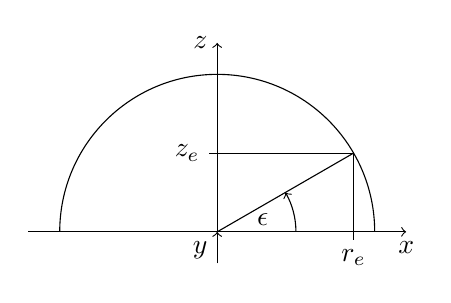
\begin{tikzpicture}[scale=2]
    \draw[->] (-1.2,0) -- (1.2,0) node[anchor=north] {$x$};
    \draw[->] (0,0) -- (0,1.2) node[anchor=east] {$z$};
    \draw[->] (0,-0.2) -- (0,0) node[anchor=north east] {$y$};
    \draw (0:1) arc (0:180:1);
    \draw (0:0) -- (30:1); 
    \draw[->] (0:0.5) arc (0:30:0.5);
    \node at (15:0.3) {$\epsilon$};
    \draw (-0.05,{sin(30)}) -- ({cos(30)},{sin(30)}) -- ({cos(30)},-0.05); 
    \node[anchor=east] at (-0.05,{sin(30)}) {$z_e$};
    \node[anchor=north] at ({cos(30)},-0.05) {$r_e$};
  \end{tikzpicture}
  \caption{Illustration of $z$-coordinate and radius of an elevated circle on
  a sphere}
  \label{fig:elevCirc}
\end{center}
\end{figure}

\noindent
Note that we actually \emph{draw} this circle in the rotated \emph{and offset}
coordinate system where it takes the form
\begin{equation}
  \begin{pmatrix} x(\varphi) \\ y(\varphi) \\ z(\varphi) \end{pmatrix}
  = \begin{pmatrix} r_e\cos\varphi \\ r_e\sin\varphi \\ {\CORR{0}} \end{pmatrix}\!.
\end{equation}
However, we will stick to Eqn.\,(\ref{eqn:csparametric}) for simplicity. The
screen coordinates for Eqn.\,(\ref{eqn:csparametric}) are
\begin{align}
  \begin{pmatrix} x'(\varphi) \\ y'(\varphi) \\ z'(\varphi) \end{pmatrix}
  &= A \begin{pmatrix} x(\varphi) \\ y(\varphi) \\ z(\varphi) \end{pmatrix}
   = \begin{pmatrix}
       a_{xx} & a_{xy} & a_{xz} \\
       a_{yx} & a_{yy} & a_{yz} \\ 
       a_{zx} & a_{zy} & a_{zz} 
     \end{pmatrix}
     \begin{pmatrix} 
       r\cos\epsilon\cos\varphi \\ 
       r\cos\epsilon\sin\varphi \\ 
       r\sin\epsilon
     \end{pmatrix}
\\
  \notag
  &= \begin{pmatrix}
       a_{xx}\cdot r\cos\epsilon\cos\varphi + a_{xy}\cdot r\cos\epsilon\sin\varphi + a_{xz}\cdot r\sin\epsilon \\
       a_{yx}\cdot r\cos\epsilon\cos\varphi + a_{yy}\cdot r\cos\epsilon\sin\varphi + a_{yz}\cdot r\sin\epsilon \\
       a_{zx}\cdot r\cos\epsilon\cos\varphi + a_{zy}\cdot r\cos\epsilon\sin\varphi + a_{zz}\cdot r\sin\epsilon
     \end{pmatrix}\!\!.
\end{align}
The $z'(\varphi)$ coordinates are not plotted. However, they are useful for
determining which parts of the circle are
\begin{align}
  \text{on the front side} &\quad z'(\varphi)\geq 0 \quad\text{and}\\
  \text{on the back side}  &\quad z'(\varphi)< 0\notag
\end{align}
of the sphere. We denote by $\varphi_0$ the crossing angles between the front
and back sides. In order to determine them we solve
\begin{align}\label{eqn:phi0}
  0
  \stackrel{!}{=} z'(\varphi_0)
  &= a_{zx}\cdot r\cos\epsilon\cos\varphi_0 
   + a_{zy}\cdot r\cos\epsilon\sin\varphi_0 
   + a_{zz}\cdot r\sin\epsilon.
\end{align}
I must admit that I was too lazy to puzzle this out myself\ldots ;-\!) Matlab
says:
\begin{align}
  \tan\left(\frac{\varphi_0}{2}\right)
  &=\frac{a_{zy}\cos\epsilon \pm \sqrt{a_{zx}^2\cos^2\epsilon + a_{zy}^2\cos^2\epsilon - a_{zz}^2\sin^2\epsilon}}
         {a_{zx}\cos\epsilon - a_{zz}\sin\epsilon}
\\
  &=\frac{a_{zy} \pm \sqrt{a_{zx}^2 + a_{zy}^2 - a_{zz}^2\tan^2\epsilon}}
         {a_{zx} - a_{zz}\tan\epsilon},
\end{align}
where
\begin{equation}
  \label{eqn:phi0cond}
  a_{zz}^2\sin^2\epsilon \ge (a_{zx}^2 + a_{zy}^2)\cos^2\epsilon
  \quad\leadsto\quad
  \tan^2\epsilon \ge \frac{a_{zx}^2 + a_{zy}^2}{a_{zz}^2}
\end{equation}
must hold. With the substitutions
\begin{align}
   u &= a_{zy}, \\ 
   v &= \sqrt{a_{zx}^2 + a_{zy}^2 - a_{zz}^2\tan^2\epsilon}\quad\text{and} \\ 
   w &= a_{zx} - a_{zz}\tan\epsilon 
\intertext{we get}
  \tan\left(\frac{\varphi_0}{2}\right)
  &=\frac{u \pm v}{w}
  \quad\leadsto\quad
  \varphi_0 = \begin{cases}
    2\atann(u+v,w)\\
    2\atann(u-v,w)  
  \end{cases}
\end{align}
Here we used the $\atann(x,y)$ function which is defined as
\begin{equation}\label{eqn:atann}
  \atann(x,y)
  = \left\{\begin{array}{ll}
      \arctan\big(\frac{x}{y}\big)     &\quad y>0          \\[5pt]
      \arctan\big(\frac{x}{y}\big)+\pi &\quad y<0, x\geq 0 \\[5pt]
      \arctan\big(\frac{x}{y}\big)-\pi &\quad y<0, x<0     \\[5pt]
      \frac{\pi}{2}                    &\quad y=0, x>0     \\[5pt]
      -\frac{\pi}{2}                   &\quad y=0, x<0     \\[5pt]
      0                                &\quad y=0, x=0
    \end{array}\right.
\end{equation}
Iff condition\,(\ref{eqn:phi0cond}) holds, Eqn.\,(\ref{eqn:phi0}) has
exactly two solutions,\footnote{which coincide iff the left and right sides of
condition \,(\ref{eqn:phi0cond}) are equal}
\begin{align}
  \varphi_{0,\text{bf}} &: \text{angle of back to front side crossing and}\notag\\
  \varphi_{0,\text{fb}} &: \text{angle of front to back side crossing,}\notag
\end{align}
Otherwise it has no solutions, which means that the circle lies entirely either
on the front side or on the back side of the sphere.

\subsection{The Package Source Code}
\lstinputlisting[style=lstsLatex,linewidth=483pt]{tikz-3dplot-circleofsphere.sty}

\subsection{An Auxiliary Matlab Script}
\lstinputlisting[style=lstsMatlab,linewidth=483pt]{tikz_3dplot_circleofsphere.m}

\addcontentsline{toc}{section}{References}
\bibliographystyle{plain}
\bibliography{tikz-3dplot-circleofsphere}

\IfFileExists{_tester.tex}{
  \clearpage
  \LTXinputExample[style=lstsFrontPage]{_tester}
}{}

\end{document}

%% EOF